
    




    
\documentclass{vgtc}

  \pdfoutput=1\relax                   % create PDFs from pdfLaTeX
  \pdfcompresslevel=9                  % PDF Compression
  \pdfoptionpdfminorversion=7          % create PDF 1.7
  \ExecuteOptions{pdftex}
  \usepackage{graphicx}                % allow us to embed graphics files


%% it is recomended to use ``\autoref{sec:bla}'' instead of ``Fig.~\ref{sec:bla}''
\graphicspath{{figures/}{pictures/}{images/}{./}} % where to search for the images

\usepackage{microtype}                 % use micro-typography (slightly more compact, better to read)
\PassOptionsToPackage{warn}{textcomp}  % to address font issues with \textrightarrow
\usepackage{textcomp}                  % use better special symbols
\usepackage{mathptmx}                  % use matching math font
\usepackage{times}                     % we use Times as the main font
\renewcommand*\ttdefault{txtt}         % a nicer typewriter font
\usepackage{cite}                      % needed to automatically sort the references
\usepackage{tabu}                      % only used for the table example
\usepackage{booktabs}                  % only used for the table example
\usepackage{multirow}
\usepackage{caption}
\usepackage{color}
\captionsetup{labelformat=default}

    
    \usepackage[breakable]{tcolorbox}
    \tcbset{nobeforeafter} % prevents tcolorboxes being placing in paragraphs
    \usepackage{float}
    \floatplacement{figure}{H} % forces figures to be placed at the correct location
    
    \usepackage[T1]{fontenc}
    % Nicer default font (+ math font) than Computer Modern for most use cases
    \usepackage{mathpazo}

    % Basic figure setup, for now with no caption control since it's done
    % automatically by Pandoc (which extracts ![](path) syntax from Markdown).
    \usepackage{graphicx}
    % We will generate all images so they have a width \maxwidth. This means
    % that they will get their normal width if they fit onto the page, but
    % are scaled down if they would overflow the margins.
    \makeatletter
    \def\maxwidth{\ifdim\Gin@nat@width>\linewidth\linewidth
    \else\Gin@nat@width\fi}
    \makeatother
    \let\Oldincludegraphics\includegraphics
    % Set max figure width to be 80% of text width, for now hardcoded.
    \renewcommand{\includegraphics}[1]{\Oldincludegraphics[width=.8\maxwidth]{#1}}
    % Ensure that by default, figures have no caption (until we provide a
    % proper Figure object with a Caption API and a way to capture that
    % in the conversion process - todo).
    \usepackage{caption}
    \DeclareCaptionLabelFormat{nolabel}{}
    \captionsetup{labelformat=nolabel}

    \usepackage{adjustbox} % Used to constrain images to a maximum size 
    \usepackage{xcolor} % Allow colors to be defined
    \usepackage{enumerate} % Needed for markdown enumerations to work
    \usepackage{geometry} % Used to adjust the document margins
    \usepackage{amsmath} % Equations
    \usepackage{amssymb} % Equations
    \usepackage{textcomp} % defines textquotesingle
    % Hack from http://tex.stackexchange.com/a/47451/13684:
    \AtBeginDocument{%
        \def\PYZsq{\textquotesingle}% Upright quotes in Pygmentized code
    }
    \usepackage{upquote} % Upright quotes for verbatim code
    \usepackage{eurosym} % defines \euro
    \usepackage[mathletters]{ucs} % Extended unicode (utf-8) support
    \usepackage[utf8x]{inputenc} % Allow utf-8 characters in the tex document
    \usepackage{fancyvrb} % verbatim replacement that allows latex
    \usepackage{grffile} % extends the file name processing of package graphics 
                         % to support a larger range 
    % The hyperref package gives us a pdf with properly built
    % internal navigation ('pdf bookmarks' for the table of contents,
    % internal cross-reference links, web links for URLs, etc.)
    \usepackage{hyperref}
    \usepackage{longtable} % longtable support required by pandoc >1.10
    \usepackage{booktabs}  % table support for pandoc > 1.12.2
    \usepackage[inline]{enumitem} % IRkernel/repr support (it uses the enumerate* environment)
    \usepackage[normalem]{ulem} % ulem is needed to support strikethroughs (\sout)
                                % normalem makes italics be italics, not underlines
    \usepackage{mathrsfs}
    

    
    % Colors for the hyperref package
    \definecolor{urlcolor}{rgb}{0,.145,.698}
    \definecolor{linkcolor}{rgb}{.71,0.21,0.01}
    \definecolor{citecolor}{rgb}{.12,.54,.11}

    % ANSI colors
    \definecolor{ansi-black}{HTML}{3E424D}
    \definecolor{ansi-black-intense}{HTML}{282C36}
    \definecolor{ansi-red}{HTML}{E75C58}
    \definecolor{ansi-red-intense}{HTML}{B22B31}
    \definecolor{ansi-green}{HTML}{00A250}
    \definecolor{ansi-green-intense}{HTML}{007427}
    \definecolor{ansi-yellow}{HTML}{DDB62B}
    \definecolor{ansi-yellow-intense}{HTML}{B27D12}
    \definecolor{ansi-blue}{HTML}{208FFB}
    \definecolor{ansi-blue-intense}{HTML}{0065CA}
    \definecolor{ansi-magenta}{HTML}{D160C4}
    \definecolor{ansi-magenta-intense}{HTML}{A03196}
    \definecolor{ansi-cyan}{HTML}{60C6C8}
    \definecolor{ansi-cyan-intense}{HTML}{258F8F}
    \definecolor{ansi-white}{HTML}{C5C1B4}
    \definecolor{ansi-white-intense}{HTML}{A1A6B2}
    \definecolor{ansi-default-inverse-fg}{HTML}{FFFFFF}
    \definecolor{ansi-default-inverse-bg}{HTML}{000000}

    % commands and environments needed by pandoc snippets
    % extracted from the output of `pandoc -s`
    \providecommand{\tightlist}{%
      \setlength{\itemsep}{0pt}\setlength{\parskip}{0pt}}
    \DefineVerbatimEnvironment{Highlighting}{Verbatim}{commandchars=\\\{\}}
    % Add ',fontsize=\small' for more characters per line
    \newenvironment{Shaded}{}{}
    \newcommand{\KeywordTok}[1]{\textcolor[rgb]{0.00,0.44,0.13}{\textbf{{#1}}}}
    \newcommand{\DataTypeTok}[1]{\textcolor[rgb]{0.56,0.13,0.00}{{#1}}}
    \newcommand{\DecValTok}[1]{\textcolor[rgb]{0.25,0.63,0.44}{{#1}}}
    \newcommand{\BaseNTok}[1]{\textcolor[rgb]{0.25,0.63,0.44}{{#1}}}
    \newcommand{\FloatTok}[1]{\textcolor[rgb]{0.25,0.63,0.44}{{#1}}}
    \newcommand{\CharTok}[1]{\textcolor[rgb]{0.25,0.44,0.63}{{#1}}}
    \newcommand{\StringTok}[1]{\textcolor[rgb]{0.25,0.44,0.63}{{#1}}}
    \newcommand{\CommentTok}[1]{\textcolor[rgb]{0.38,0.63,0.69}{\textit{{#1}}}}
    \newcommand{\OtherTok}[1]{\textcolor[rgb]{0.00,0.44,0.13}{{#1}}}
    \newcommand{\AlertTok}[1]{\textcolor[rgb]{1.00,0.00,0.00}{\textbf{{#1}}}}
    \newcommand{\FunctionTok}[1]{\textcolor[rgb]{0.02,0.16,0.49}{{#1}}}
    \newcommand{\RegionMarkerTok}[1]{{#1}}
    \newcommand{\ErrorTok}[1]{\textcolor[rgb]{1.00,0.00,0.00}{\textbf{{#1}}}}
    \newcommand{\NormalTok}[1]{{#1}}
    
    % Additional commands for more recent versions of Pandoc
    \newcommand{\ConstantTok}[1]{\textcolor[rgb]{0.53,0.00,0.00}{{#1}}}
    \newcommand{\SpecialCharTok}[1]{\textcolor[rgb]{0.25,0.44,0.63}{{#1}}}
    \newcommand{\VerbatimStringTok}[1]{\textcolor[rgb]{0.25,0.44,0.63}{{#1}}}
    \newcommand{\SpecialStringTok}[1]{\textcolor[rgb]{0.73,0.40,0.53}{{#1}}}
    \newcommand{\ImportTok}[1]{{#1}}
    \newcommand{\DocumentationTok}[1]{\textcolor[rgb]{0.73,0.13,0.13}{\textit{{#1}}}}
    \newcommand{\AnnotationTok}[1]{\textcolor[rgb]{0.38,0.63,0.69}{\textbf{\textit{{#1}}}}}
    \newcommand{\CommentVarTok}[1]{\textcolor[rgb]{0.38,0.63,0.69}{\textbf{\textit{{#1}}}}}
    \newcommand{\VariableTok}[1]{\textcolor[rgb]{0.10,0.09,0.49}{{#1}}}
    \newcommand{\ControlFlowTok}[1]{\textcolor[rgb]{0.00,0.44,0.13}{\textbf{{#1}}}}
    \newcommand{\OperatorTok}[1]{\textcolor[rgb]{0.40,0.40,0.40}{{#1}}}
    \newcommand{\BuiltInTok}[1]{{#1}}
    \newcommand{\ExtensionTok}[1]{{#1}}
    \newcommand{\PreprocessorTok}[1]{\textcolor[rgb]{0.74,0.48,0.00}{{#1}}}
    \newcommand{\AttributeTok}[1]{\textcolor[rgb]{0.49,0.56,0.16}{{#1}}}
    \newcommand{\InformationTok}[1]{\textcolor[rgb]{0.38,0.63,0.69}{\textbf{\textit{{#1}}}}}
    \newcommand{\WarningTok}[1]{\textcolor[rgb]{0.38,0.63,0.69}{\textbf{\textit{{#1}}}}}
    
    
    % Define a nice break command that doesn't care if a line doesn't already
    % exist.
    \def\br{\hspace*{\fill} \\* }
    % Math Jax compatibility definitions
    \def\gt{>}
    \def\lt{<}
    \let\Oldtex\TeX
    \let\Oldlatex\LaTeX
    \renewcommand{\TeX}{\textrm{\Oldtex}}
    \renewcommand{\LaTeX}{\textrm{\Oldlatex}}
    % Document parameters
    % Document title
    \title{MotionRetargetingPaper-3}
    
    
    
    
    
% Pygments definitions
\makeatletter
\def\PY@reset{\let\PY@it=\relax \let\PY@bf=\relax%
    \let\PY@ul=\relax \let\PY@tc=\relax%
    \let\PY@bc=\relax \let\PY@ff=\relax}
\def\PY@tok#1{\csname PY@tok@#1\endcsname}
\def\PY@toks#1+{\ifx\relax#1\empty\else%
    \PY@tok{#1}\expandafter\PY@toks\fi}
\def\PY@do#1{\PY@bc{\PY@tc{\PY@ul{%
    \PY@it{\PY@bf{\PY@ff{#1}}}}}}}
\def\PY#1#2{\PY@reset\PY@toks#1+\relax+\PY@do{#2}}

\expandafter\def\csname PY@tok@w\endcsname{\def\PY@tc##1{\textcolor[rgb]{0.73,0.73,0.73}{##1}}}
\expandafter\def\csname PY@tok@c\endcsname{\let\PY@it=\textit\def\PY@tc##1{\textcolor[rgb]{0.25,0.50,0.50}{##1}}}
\expandafter\def\csname PY@tok@cp\endcsname{\def\PY@tc##1{\textcolor[rgb]{0.74,0.48,0.00}{##1}}}
\expandafter\def\csname PY@tok@k\endcsname{\let\PY@bf=\textbf\def\PY@tc##1{\textcolor[rgb]{0.00,0.50,0.00}{##1}}}
\expandafter\def\csname PY@tok@kp\endcsname{\def\PY@tc##1{\textcolor[rgb]{0.00,0.50,0.00}{##1}}}
\expandafter\def\csname PY@tok@kt\endcsname{\def\PY@tc##1{\textcolor[rgb]{0.69,0.00,0.25}{##1}}}
\expandafter\def\csname PY@tok@o\endcsname{\def\PY@tc##1{\textcolor[rgb]{0.40,0.40,0.40}{##1}}}
\expandafter\def\csname PY@tok@ow\endcsname{\let\PY@bf=\textbf\def\PY@tc##1{\textcolor[rgb]{0.67,0.13,1.00}{##1}}}
\expandafter\def\csname PY@tok@nb\endcsname{\def\PY@tc##1{\textcolor[rgb]{0.00,0.50,0.00}{##1}}}
\expandafter\def\csname PY@tok@nf\endcsname{\def\PY@tc##1{\textcolor[rgb]{0.00,0.00,1.00}{##1}}}
\expandafter\def\csname PY@tok@nc\endcsname{\let\PY@bf=\textbf\def\PY@tc##1{\textcolor[rgb]{0.00,0.00,1.00}{##1}}}
\expandafter\def\csname PY@tok@nn\endcsname{\let\PY@bf=\textbf\def\PY@tc##1{\textcolor[rgb]{0.00,0.00,1.00}{##1}}}
\expandafter\def\csname PY@tok@ne\endcsname{\let\PY@bf=\textbf\def\PY@tc##1{\textcolor[rgb]{0.82,0.25,0.23}{##1}}}
\expandafter\def\csname PY@tok@nv\endcsname{\def\PY@tc##1{\textcolor[rgb]{0.10,0.09,0.49}{##1}}}
\expandafter\def\csname PY@tok@no\endcsname{\def\PY@tc##1{\textcolor[rgb]{0.53,0.00,0.00}{##1}}}
\expandafter\def\csname PY@tok@nl\endcsname{\def\PY@tc##1{\textcolor[rgb]{0.63,0.63,0.00}{##1}}}
\expandafter\def\csname PY@tok@ni\endcsname{\let\PY@bf=\textbf\def\PY@tc##1{\textcolor[rgb]{0.60,0.60,0.60}{##1}}}
\expandafter\def\csname PY@tok@na\endcsname{\def\PY@tc##1{\textcolor[rgb]{0.49,0.56,0.16}{##1}}}
\expandafter\def\csname PY@tok@nt\endcsname{\let\PY@bf=\textbf\def\PY@tc##1{\textcolor[rgb]{0.00,0.50,0.00}{##1}}}
\expandafter\def\csname PY@tok@nd\endcsname{\def\PY@tc##1{\textcolor[rgb]{0.67,0.13,1.00}{##1}}}
\expandafter\def\csname PY@tok@s\endcsname{\def\PY@tc##1{\textcolor[rgb]{0.73,0.13,0.13}{##1}}}
\expandafter\def\csname PY@tok@sd\endcsname{\let\PY@it=\textit\def\PY@tc##1{\textcolor[rgb]{0.73,0.13,0.13}{##1}}}
\expandafter\def\csname PY@tok@si\endcsname{\let\PY@bf=\textbf\def\PY@tc##1{\textcolor[rgb]{0.73,0.40,0.53}{##1}}}
\expandafter\def\csname PY@tok@se\endcsname{\let\PY@bf=\textbf\def\PY@tc##1{\textcolor[rgb]{0.73,0.40,0.13}{##1}}}
\expandafter\def\csname PY@tok@sr\endcsname{\def\PY@tc##1{\textcolor[rgb]{0.73,0.40,0.53}{##1}}}
\expandafter\def\csname PY@tok@ss\endcsname{\def\PY@tc##1{\textcolor[rgb]{0.10,0.09,0.49}{##1}}}
\expandafter\def\csname PY@tok@sx\endcsname{\def\PY@tc##1{\textcolor[rgb]{0.00,0.50,0.00}{##1}}}
\expandafter\def\csname PY@tok@m\endcsname{\def\PY@tc##1{\textcolor[rgb]{0.40,0.40,0.40}{##1}}}
\expandafter\def\csname PY@tok@gh\endcsname{\let\PY@bf=\textbf\def\PY@tc##1{\textcolor[rgb]{0.00,0.00,0.50}{##1}}}
\expandafter\def\csname PY@tok@gu\endcsname{\let\PY@bf=\textbf\def\PY@tc##1{\textcolor[rgb]{0.50,0.00,0.50}{##1}}}
\expandafter\def\csname PY@tok@gd\endcsname{\def\PY@tc##1{\textcolor[rgb]{0.63,0.00,0.00}{##1}}}
\expandafter\def\csname PY@tok@gi\endcsname{\def\PY@tc##1{\textcolor[rgb]{0.00,0.63,0.00}{##1}}}
\expandafter\def\csname PY@tok@gr\endcsname{\def\PY@tc##1{\textcolor[rgb]{1.00,0.00,0.00}{##1}}}
\expandafter\def\csname PY@tok@ge\endcsname{\let\PY@it=\textit}
\expandafter\def\csname PY@tok@gs\endcsname{\let\PY@bf=\textbf}
\expandafter\def\csname PY@tok@gp\endcsname{\let\PY@bf=\textbf\def\PY@tc##1{\textcolor[rgb]{0.00,0.00,0.50}{##1}}}
\expandafter\def\csname PY@tok@go\endcsname{\def\PY@tc##1{\textcolor[rgb]{0.53,0.53,0.53}{##1}}}
\expandafter\def\csname PY@tok@gt\endcsname{\def\PY@tc##1{\textcolor[rgb]{0.00,0.27,0.87}{##1}}}
\expandafter\def\csname PY@tok@err\endcsname{\def\PY@bc##1{\setlength{\fboxsep}{0pt}\fcolorbox[rgb]{1.00,0.00,0.00}{1,1,1}{\strut ##1}}}
\expandafter\def\csname PY@tok@kc\endcsname{\let\PY@bf=\textbf\def\PY@tc##1{\textcolor[rgb]{0.00,0.50,0.00}{##1}}}
\expandafter\def\csname PY@tok@kd\endcsname{\let\PY@bf=\textbf\def\PY@tc##1{\textcolor[rgb]{0.00,0.50,0.00}{##1}}}
\expandafter\def\csname PY@tok@kn\endcsname{\let\PY@bf=\textbf\def\PY@tc##1{\textcolor[rgb]{0.00,0.50,0.00}{##1}}}
\expandafter\def\csname PY@tok@kr\endcsname{\let\PY@bf=\textbf\def\PY@tc##1{\textcolor[rgb]{0.00,0.50,0.00}{##1}}}
\expandafter\def\csname PY@tok@bp\endcsname{\def\PY@tc##1{\textcolor[rgb]{0.00,0.50,0.00}{##1}}}
\expandafter\def\csname PY@tok@fm\endcsname{\def\PY@tc##1{\textcolor[rgb]{0.00,0.00,1.00}{##1}}}
\expandafter\def\csname PY@tok@vc\endcsname{\def\PY@tc##1{\textcolor[rgb]{0.10,0.09,0.49}{##1}}}
\expandafter\def\csname PY@tok@vg\endcsname{\def\PY@tc##1{\textcolor[rgb]{0.10,0.09,0.49}{##1}}}
\expandafter\def\csname PY@tok@vi\endcsname{\def\PY@tc##1{\textcolor[rgb]{0.10,0.09,0.49}{##1}}}
\expandafter\def\csname PY@tok@vm\endcsname{\def\PY@tc##1{\textcolor[rgb]{0.10,0.09,0.49}{##1}}}
\expandafter\def\csname PY@tok@sa\endcsname{\def\PY@tc##1{\textcolor[rgb]{0.73,0.13,0.13}{##1}}}
\expandafter\def\csname PY@tok@sb\endcsname{\def\PY@tc##1{\textcolor[rgb]{0.73,0.13,0.13}{##1}}}
\expandafter\def\csname PY@tok@sc\endcsname{\def\PY@tc##1{\textcolor[rgb]{0.73,0.13,0.13}{##1}}}
\expandafter\def\csname PY@tok@dl\endcsname{\def\PY@tc##1{\textcolor[rgb]{0.73,0.13,0.13}{##1}}}
\expandafter\def\csname PY@tok@s2\endcsname{\def\PY@tc##1{\textcolor[rgb]{0.73,0.13,0.13}{##1}}}
\expandafter\def\csname PY@tok@sh\endcsname{\def\PY@tc##1{\textcolor[rgb]{0.73,0.13,0.13}{##1}}}
\expandafter\def\csname PY@tok@s1\endcsname{\def\PY@tc##1{\textcolor[rgb]{0.73,0.13,0.13}{##1}}}
\expandafter\def\csname PY@tok@mb\endcsname{\def\PY@tc##1{\textcolor[rgb]{0.40,0.40,0.40}{##1}}}
\expandafter\def\csname PY@tok@mf\endcsname{\def\PY@tc##1{\textcolor[rgb]{0.40,0.40,0.40}{##1}}}
\expandafter\def\csname PY@tok@mh\endcsname{\def\PY@tc##1{\textcolor[rgb]{0.40,0.40,0.40}{##1}}}
\expandafter\def\csname PY@tok@mi\endcsname{\def\PY@tc##1{\textcolor[rgb]{0.40,0.40,0.40}{##1}}}
\expandafter\def\csname PY@tok@il\endcsname{\def\PY@tc##1{\textcolor[rgb]{0.40,0.40,0.40}{##1}}}
\expandafter\def\csname PY@tok@mo\endcsname{\def\PY@tc##1{\textcolor[rgb]{0.40,0.40,0.40}{##1}}}
\expandafter\def\csname PY@tok@ch\endcsname{\let\PY@it=\textit\def\PY@tc##1{\textcolor[rgb]{0.25,0.50,0.50}{##1}}}
\expandafter\def\csname PY@tok@cm\endcsname{\let\PY@it=\textit\def\PY@tc##1{\textcolor[rgb]{0.25,0.50,0.50}{##1}}}
\expandafter\def\csname PY@tok@cpf\endcsname{\let\PY@it=\textit\def\PY@tc##1{\textcolor[rgb]{0.25,0.50,0.50}{##1}}}
\expandafter\def\csname PY@tok@c1\endcsname{\let\PY@it=\textit\def\PY@tc##1{\textcolor[rgb]{0.25,0.50,0.50}{##1}}}
\expandafter\def\csname PY@tok@cs\endcsname{\let\PY@it=\textit\def\PY@tc##1{\textcolor[rgb]{0.25,0.50,0.50}{##1}}}

\def\PYZbs{\char`\\}
\def\PYZus{\char`\_}
\def\PYZob{\char`\{}
\def\PYZcb{\char`\}}
\def\PYZca{\char`\^}
\def\PYZam{\char`\&}
\def\PYZlt{\char`\<}
\def\PYZgt{\char`\>}
\def\PYZsh{\char`\#}
\def\PYZpc{\char`\%}
\def\PYZdl{\char`\$}
\def\PYZhy{\char`\-}
\def\PYZsq{\char`\'}
\def\PYZdq{\char`\"}
\def\PYZti{\char`\~}
% for compatibility with earlier versions
\def\PYZat{@}
\def\PYZlb{[}
\def\PYZrb{]}
\makeatother


    % For linebreaks inside Verbatim environment from package fancyvrb. 
    \makeatletter
        \newbox\Wrappedcontinuationbox 
        \newbox\Wrappedvisiblespacebox 
        \newcommand*\Wrappedvisiblespace {\textcolor{red}{\textvisiblespace}} 
        \newcommand*\Wrappedcontinuationsymbol {\textcolor{red}{\llap{\tiny$\m@th\hookrightarrow$}}} 
        \newcommand*\Wrappedcontinuationindent {3ex } 
        \newcommand*\Wrappedafterbreak {\kern\Wrappedcontinuationindent\copy\Wrappedcontinuationbox} 
        % Take advantage of the already applied Pygments mark-up to insert 
        % potential linebreaks for TeX processing. 
        %        {, <, #, %, $, ' and ": go to next line. 
        %        _, }, ^, &, >, - and ~: stay at end of broken line. 
        % Use of \textquotesingle for straight quote. 
        \newcommand*\Wrappedbreaksatspecials {% 
            \def\PYGZus{\discretionary{\char`\_}{\Wrappedafterbreak}{\char`\_}}% 
            \def\PYGZob{\discretionary{}{\Wrappedafterbreak\char`\{}{\char`\{}}% 
            \def\PYGZcb{\discretionary{\char`\}}{\Wrappedafterbreak}{\char`\}}}% 
            \def\PYGZca{\discretionary{\char`\^}{\Wrappedafterbreak}{\char`\^}}% 
            \def\PYGZam{\discretionary{\char`\&}{\Wrappedafterbreak}{\char`\&}}% 
            \def\PYGZlt{\discretionary{}{\Wrappedafterbreak\char`\<}{\char`\<}}% 
            \def\PYGZgt{\discretionary{\char`\>}{\Wrappedafterbreak}{\char`\>}}% 
            \def\PYGZsh{\discretionary{}{\Wrappedafterbreak\char`\#}{\char`\#}}% 
            \def\PYGZpc{\discretionary{}{\Wrappedafterbreak\char`\%}{\char`\%}}% 
            \def\PYGZdl{\discretionary{}{\Wrappedafterbreak\char`\$}{\char`\$}}% 
            \def\PYGZhy{\discretionary{\char`\-}{\Wrappedafterbreak}{\char`\-}}% 
            \def\PYGZsq{\discretionary{}{\Wrappedafterbreak\textquotesingle}{\textquotesingle}}% 
            \def\PYGZdq{\discretionary{}{\Wrappedafterbreak\char`\"}{\char`\"}}% 
            \def\PYGZti{\discretionary{\char`\~}{\Wrappedafterbreak}{\char`\~}}% 
        } 
        % Some characters . , ; ? ! / are not pygmentized. 
        % This macro makes them "active" and they will insert potential linebreaks 
        \newcommand*\Wrappedbreaksatpunct {% 
            \lccode`\~`\.\lowercase{\def~}{\discretionary{\hbox{\char`\.}}{\Wrappedafterbreak}{\hbox{\char`\.}}}% 
            \lccode`\~`\,\lowercase{\def~}{\discretionary{\hbox{\char`\,}}{\Wrappedafterbreak}{\hbox{\char`\,}}}% 
            \lccode`\~`\;\lowercase{\def~}{\discretionary{\hbox{\char`\;}}{\Wrappedafterbreak}{\hbox{\char`\;}}}% 
            \lccode`\~`\:\lowercase{\def~}{\discretionary{\hbox{\char`\:}}{\Wrappedafterbreak}{\hbox{\char`\:}}}% 
            \lccode`\~`\?\lowercase{\def~}{\discretionary{\hbox{\char`\?}}{\Wrappedafterbreak}{\hbox{\char`\?}}}% 
            \lccode`\~`\!\lowercase{\def~}{\discretionary{\hbox{\char`\!}}{\Wrappedafterbreak}{\hbox{\char`\!}}}% 
            \lccode`\~`\/\lowercase{\def~}{\discretionary{\hbox{\char`\/}}{\Wrappedafterbreak}{\hbox{\char`\/}}}% 
            \catcode`\.\active
            \catcode`\,\active 
            \catcode`\;\active
            \catcode`\:\active
            \catcode`\?\active
            \catcode`\!\active
            \catcode`\/\active 
            \lccode`\~`\~ 	
        }
    \makeatother

    \let\OriginalVerbatim=\Verbatim
    \makeatletter
    \renewcommand{\Verbatim}[1][1]{%
        %\parskip\z@skip
        \sbox\Wrappedcontinuationbox {\Wrappedcontinuationsymbol}%
        \sbox\Wrappedvisiblespacebox {\FV@SetupFont\Wrappedvisiblespace}%
        \def\FancyVerbFormatLine ##1{\hsize\linewidth
            \vtop{\raggedright\hyphenpenalty\z@\exhyphenpenalty\z@
                \doublehyphendemerits\z@\finalhyphendemerits\z@
                \strut ##1\strut}%
        }%
        % If the linebreak is at a space, the latter will be displayed as visible
        % space at end of first line, and a continuation symbol starts next line.
        % Stretch/shrink are however usually zero for typewriter font.
        \def\FV@Space {%
            \nobreak\hskip\z@ plus\fontdimen3\font minus\fontdimen4\font
            \discretionary{\copy\Wrappedvisiblespacebox}{\Wrappedafterbreak}
            {\kern\fontdimen2\font}%
        }%
        
        % Allow breaks at special characters using \PYG... macros.
        \Wrappedbreaksatspecials
        % Breaks at punctuation characters . , ; ? ! and / need catcode=\active 	
        \OriginalVerbatim[#1,codes*=\Wrappedbreaksatpunct]%
    }
    \makeatother

    % Exact colors from NB
    \definecolor{incolor}{HTML}{303F9F}
    \definecolor{outcolor}{HTML}{D84315}
    \definecolor{cellborder}{HTML}{CFCFCF}
    \definecolor{cellbackground}{HTML}{F7F7F7}
    
    % prompt
    \newcommand{\prompt}[4]{
        \llap{{\color{#2}[#3]: #4}}\vspace{-1.25em}
    }
    

    
    % Prevent overflowing lines due to hard-to-break entities
    \sloppy 
    % Setup hyperref package
    \hypersetup{
      breaklinks=true,  % so long urls are correctly broken across lines
      colorlinks=true,
      urlcolor=urlcolor,
      linkcolor=linkcolor,
      citecolor=citecolor,
      }
    % Slightly bigger margins than the latex defaults
    
    \geometry{verbose,tmargin=1in,bmargin=1in,lmargin=1in,rmargin=1in}
    
    

    \begin{document}
    
    
    \author{Rodolfo L. Tonoli \thanks{ e-mail: rltonoli@gmail.com }}\affiliation{Department of Computer Engineering and Industrial Automation\\School of Electrical and Computer Engineering\\University of Campinas}\title{Motion Capture Retargeting: Preserving Surface Spatial Relationship}\keywords{Motion Capture, Motion Retargeting, 3D Animation, Virtual Agents.}\CCScatlist{\CCScat{Computing methodologies}{Computer graphics}{Animation}{Motion capture}}\abstract{ Motion Capture is used to record the movements of a real actor and animate virtual characters. It generates intrinsically realistic animations, since it tracks the motion of a real person. But the process to transfer the motion to a character is not straigthforward since the actor and the character may have distinct body proportions and distinct skeleton topology. The present work focus on retargeting the motion from Motion Capture to a 3D character while preserving the spatial relationship betweeen extremity joints, the hands and the feet, and the body surface. This process retain the semantic information information of movements in which the hands and the feet interact with the surface of the body, as holding the hands in front of the eyes or mouth. The Motion Retargeting process described computes new positions of the extremity joints regarding surface components of the body and adapts the pose of the virtual character in the posistions computed using Inverse Kinematics. The motion can be transfered to topologically different skeletons. The results shows that the resulting motion is being adapted accordingly to the body surface and it is as smooth as the original motion capture data.}
   
\maketitle
\captionsetup{labelformat=default}

    
    

    
    \section{Introduction}\label{introduction}

Toy Story was released in 1995 as the first full length film produced
entirely through computer animation techniques\cite{henne}. Besides
Pixar's production, several applications employ digital animations to
entertain, convey information, educate, among others. Some exploits the
use of virtual human models to make the human-computer interatction more
natural and accessible. Talita, the virtual human of the TAS
project\cite{demartino}, is a signing avatar that communicates with deaf
students using the Brazilian Sign Language. The goal of the TAS project
is to help the deaf and hard of hearing to access information and in
their educational process.

Humans use not only the voice and facial expression cues to understand
intentions, motives and wills, but also the movements of our body and
limbs may carry semantic information on the emotion that one is triyng
to express. The location, orientation and speed of the hand are some of
the parameters that characterizes a sign language gesture, slightly
discrepancies will express different messages or even make the gesture
unrecognizable. Therefore, an accurate motion representation by the
virtual agent should be of great concern.

Keyframing is a technique to animate an avatar, the animator adjusts
crucial poses of the 3D character on dispersed frames and an algorithm
fills the gap between two poses by interpolating them over time, which
creates the impression of the desired motion. Another digital animation
technique is Motion Capture (MoCap) that aims to lessen the
time-consuming and tedious work of keyframing animations. MoCap systems
registers an actor performing the desired motion to animate a 3D
character. Optical Motion Capture systems, for example, uses a set of
cameras to track the position over time of reflective markers placed on
the body surface of the performer. The motion is then transferred to the
avatar, the motion retargeting process, without the need to create all
the poses along the action.

The motion retargeting, however, can cause ill-conditioned poses when
the body proportions of the performer and the avatar are different. The
motion retargeting of an actor with long arms covering his ears, as an
example, to a 3D character with short arms results in a unrecognizable
action, since the hands of the avatar will not reach its ears. In this
case, the animator must inspect the animation, identify the irregular
artifacts and correct them with keyframing, adjusting the avatar pose to
the desired one. Some motion retargeting algorithms aims to avoid such
artifacts to further reduce the inspection and adjustments needed by the
animator.

    \section{Method}\label{method}

\begin{figure}
\centering
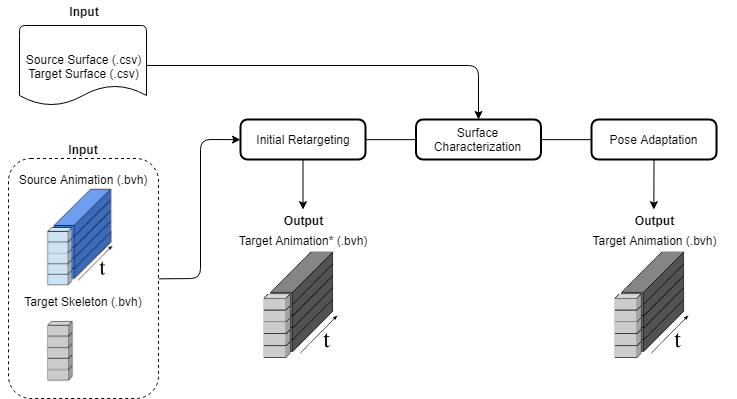
\includegraphics{../figures/Workflow3.png}
\caption{Process overview that computes the target motion given the
source motion and the target skeleton.}
\end{figure}

    \subsection{Initial Retargeting}\label{initial-retargeting}

This Section describes the Initial Motion Retargeting process, which
receives the source animation and the target skeleton as inputs, both
BVH files. The output is an animation of the target skeleton performing
the movements of the source skeleton that can be exported as a BVH file.
The success of the process does not depend on matching topologies of the
skeletons, but the first pose of the source animation and the target
skeleton pose must be as close as possible to the T-Pose. The output of
the Initial Retargeting is the target skeleton animation. The target
animation does not exploit yet the ``surface-awareness'' adjustments
that the methods described in the subsequent sections provide, but it
can already be imported in game engines or animation softwares to
animate a 3D character.

To animate a skeleton, its joints must rotate and translate along the
frames, conveying the impression of motion. The hierarchical
representation of the skeleton allows an all-around description of the
motion by only preserving the rotational and translational values of a
joint regarding its parent joint, i.e., local rotations and
translations. Given a joint \(n\) in the skeleton, its global transform
matrix \(M_{global}^{n}\) is the combination of the local transform
matrices of all the joints above the hierarchy:

\begin{equation}
\label{eq:transformmatrixglobal}
M_{global}^{n} = \prod_{i=0}^{n} M_{local}^{i}
\end{equation}

    \subsubsection{Skeleton Mapping}\label{skeleton-mapping}

Figure 2 presents two approaches to represent a virtual human skeleton.
Although both can animate a humanoid-shaped model, transferring motions
between the skeletons is not straightforward. A correspondence between
joints of the skeletons is mandatory to identify which joints from the
target skeleton should mimic the motion from the source skeleton. It is
possible to infer a correspondence using the joints' name automatically,
but note that they may not be placed at the same point in the respective
skeleton, as the shoulders in the figure. Therefore, the user can
provide a correspondence between skeletons to properly map joints and to
perform the motion retargeting\cite{hsieh}.

\begin{figure}
\centering
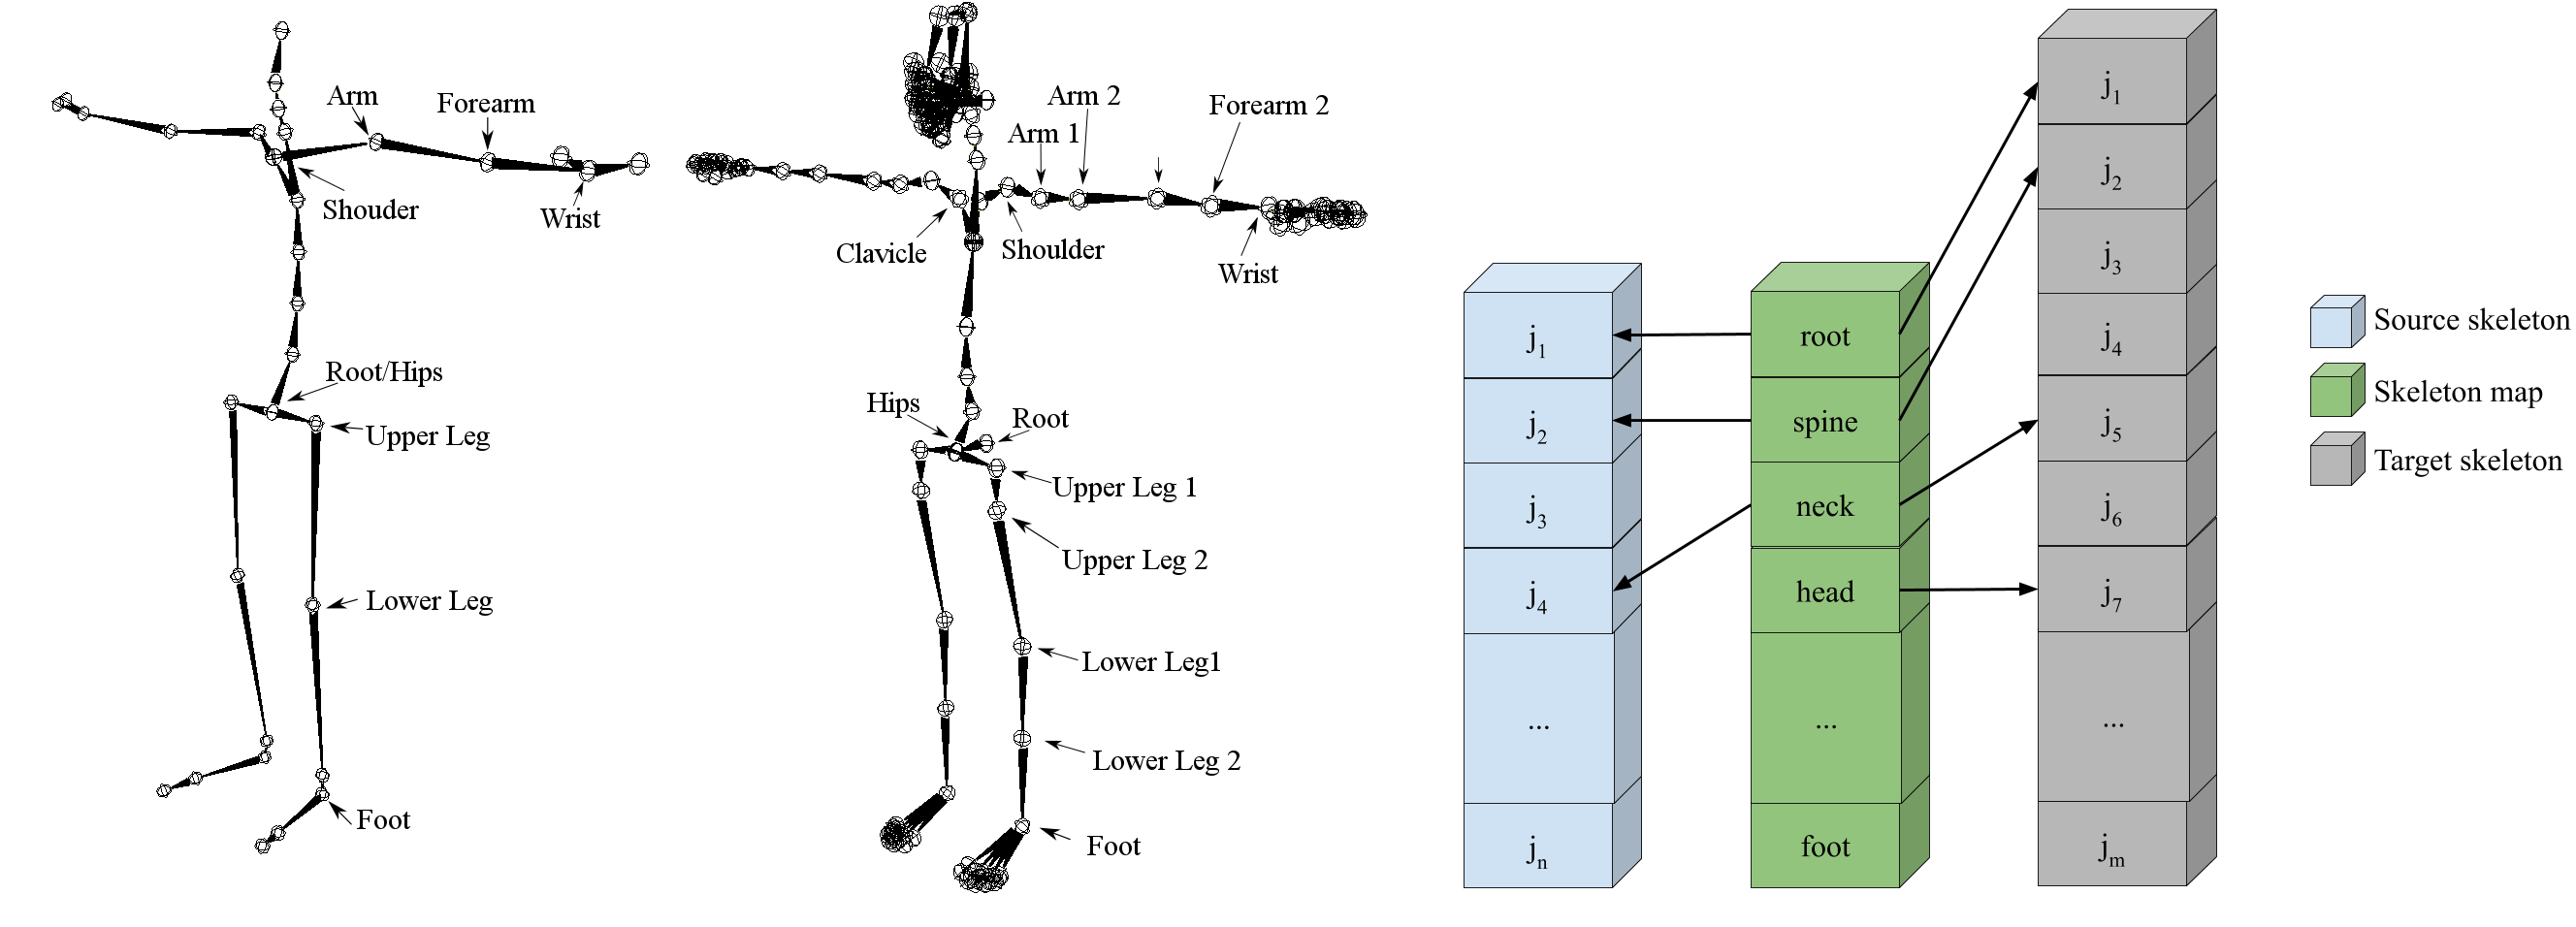
\includegraphics{../figures/skelmap.png}
\caption{Skeleton Map}
\end{figure}

In this work, it is required that both target and source skeletons have
at least the set of joints: one hips joint, three spine joints, neck and
head joints, and right and left joints for the shoulders, elbows,
wrists, femurs, knees and feet. The joints referenced will be the only
ones used in the Initial Retargeting proccess.

\subsubsection{Bones Alignment}\label{bones-alignment}

Bones Alignment enforces that the vector of a mapped joint from the
target skeleton pointing towards its child joint has the same direction
of the correspondent vector from the source skeleton. Then, for every
frame, we apply the same transform from the source skeleton joint to the
correspondent target joint.

The rotation matrix \(R_{A}\) to align the bone vector of the target
skeleton onto the bone vector of the source skeleton is calculated and
applied to the global rotation of the target skeleton joint
\(R_{G}^{n}\):

\begin{equation}
        \label{eq:newglobal}
        R_{NG}^{n} = R_{A} R_{G}^{n}
        \end{equation}

where \(R_{NG}^{n}\) is the new global rotation. Then we recover the
local rotation of the joint \(R_{L}^{n}\), the new global orientation is
multiplied by its parent inverse rotation matrix.

\begin{equation}
        \label{eq:newglobal2}
        R_{NG}^{n} = \left(\prod_{i=0}^{n-1} R_{L}^{i}\right) R_{L}^{n} 
        \end{equation}

\begin{equation}
    \label{eq:newglobal3}
    R_{NG}^{n} = R_{G}^{n-1} R_{L}^{n}
    \end{equation}

\begin{equation}
    \label{eq:newglobal4}
    R_{L}^{n} = (R_{G}^{n-1})^{-1} R_{NG}^{n}
    \end{equation}

In the following frames, the rotation of a joint in the source
animation, from the last frame to the current one, replaces the rotation
\(R_{A}\) to align the correspondent joint in the target skeleton.

We compute the ratio of the heights of the root joint from the target
and source skeletons in the first frame. The position of the root joint
in the target skeleton is adapted using Equation \ref{eq:rootmov}.

\begin{equation}
    \label{eq:rootmov}
    \mathbf{p}(t)_{tgt} = \mathbf{p}(t)_{src} ratio
    \end{equation}

    \subsection{Surface Calibration}\label{surface-calibration}

Molla\cite{molla} defined a set of points to characterize the surface of
the 3D model's and performer's body, the yellow dots in Figure 3. The
points are connected throughtriangles to create a mesh that represents
the body surface. The points on the surfaceof the character and the
performer need to be collected as close to the relative positionas
possible, since the triangle mesh differences between the characters
must represent differences of the characters' surface, thus sampling
surface points from different placesintroduces noise to the analysis.
The thickness of the limbs are also registered and later they are
represented by capsules to avoid self-penetration in the animation.

\begin{figure}
\centering
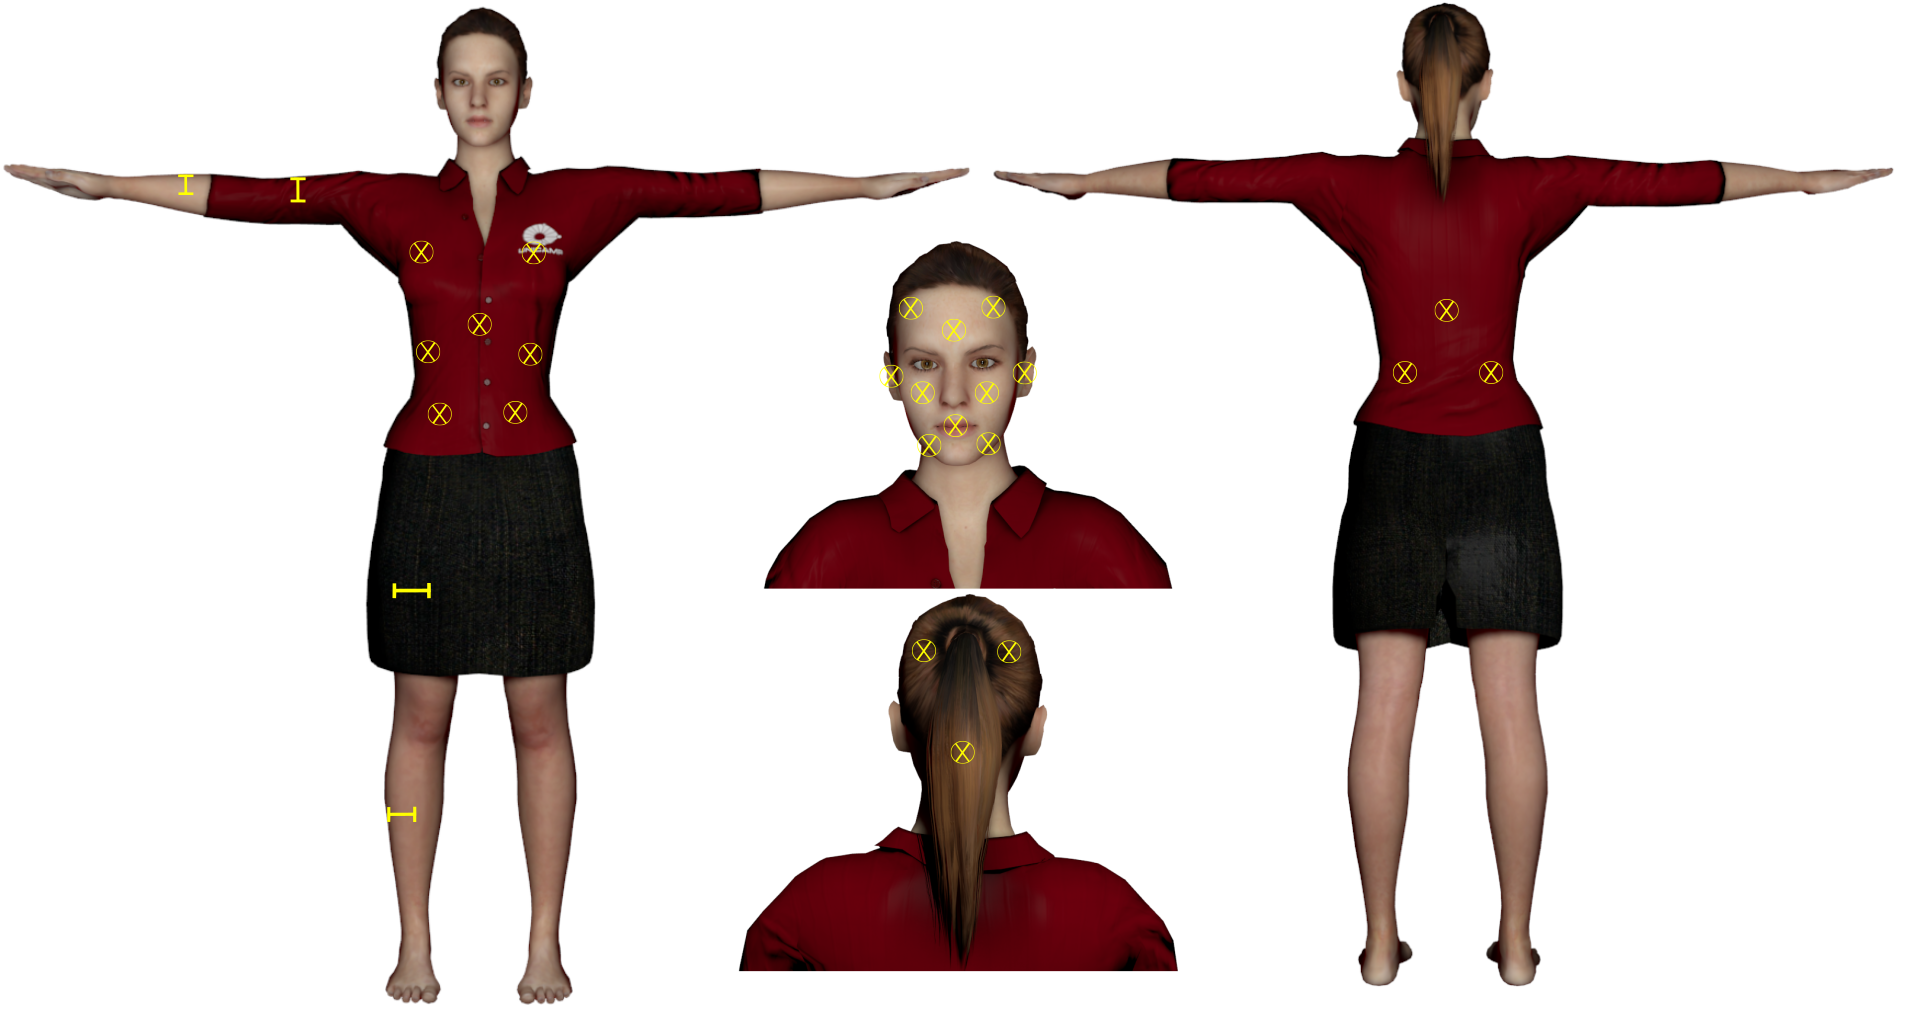
\includegraphics{../figures/TalitaPoints.png}
\caption{Surface points sampled in the 3D character for the Surface
Calibration.}
\end{figure}

The user obtains the surface points and radius of each limb of the
character during its creation or through a 3D modeling software.

    \subsubsection{Surface Motion
Estimation}\label{surface-motion-estimation}

Collecting the position of the surface points is not enough because the
performer may walk around, jump or simply twist his torso. In those
cases, the sampled points do not represent the current surface position,
since we do not keep track of these points. To include the surface
deformation - translation and twist effects - we attach each calibration
point representing the character mesh (yellow dots in Figure 3) to the
nearest mapped joint. Thus, the point behaves as a child of the mapped
joint and the transformations from every joint in the hierarchy is also
applied to the point.

    \subsection{Computing Egocentric
Coordinates}\label{computing-egocentric-coordinates}

We compute the egocentric coordinates of each limb joint in respect to
each triangle in the surface mesh and for each capsule limb. Molla
computes the projection of the joint's position \(\mathbf{p}\) on the
\(m\) triangles of the mesh, the projected point \(\mathbf{x}\) is
called the reference point, and the displacement vector \(\mathbf{v}\)
is the distance of the joint's position to the reference point. Then,
the position of joint \(n\) regarding the surface component \(i\) is
expressed as the equation:

\begin{equation}
\label{eq:egocoord_jointpos1}
\mathbf{p}_n = \mathbf{x}_i + \mathbf{v}_i
\end{equation}

The position is expressed likewise for the limbs, but the reference
point is the intersection between the capsule surface and the line that
passes through the center of the capsule and the joint's position. Then,
combining all the surface components, limbs and meshes, the previous
equation becomes:

\begin{equation}
\label{eq:egocoord_jointpos2}
\mathbf{p}_n = \sum_{i=1}^{m}\hat{\lambda}_{i}(\mathbf{x}_i + \mathbf{v}_i)
\end{equation}

The importance factor \(\lambda\) of a surface component is metric that
encodes the proximity and orthogonality between the component and the
joint's position. The goal of the importance factor is allow that
surface components that are near and more perpendicular to the joint
have a higher contribution on the joint's position calculation.

Furthermore, a small distance between the joint and the surface may
indicate that a interaction is occurring, covering the eyes with the
hand as an example. In this case, we desire that the weights of the hand
position that a surface component in head express excel the weights of
the torso surface component, in order to preserve the interaction
between the head and not with the torso.

The importance factor of a surface component is the combination of the
proximity \(\lambda_p\) and the orthogonality \(\lambda_{\perp}\)
properties:

\begin{equation}
\label{eq:importance}
\lambda = \lambda_p \lambda_{\perp}\hspace{0.1cm},\hspace{0.1cm} with \hspace{0.2cm}\lambda_p =  \frac{1}{||\mathbf{v}||}\hspace{0.2cm} and \hspace{0.2cm}\lambda_{\perp} = cos(\alpha)
\end{equation}

where \(\alpha\) is the angle between the displacement vector
\(\mathbf{v}\) and the surface component normal. Finally,
\(\hat{\lambda}_{i}\) is computed as

\begin{equation}
\label{eq:importance_ortho}
\hat{\lambda}_{i} = \frac{\lambda_{i}}{\sum_{j=1}^{m}\lambda_{j}}
\end{equation}

Using the target character surface information to compute the reference
points and the displacement vectors from the source skeleton, and
reversing Equation, we obtain the position for a target skeleton joint
with the same distance from its surface as the source skeleton distance
from its respective surface. But differences in the body proportions and
bones length between the skeletons still were not taken into account,
which will result in odd-looking poses or in a position impossible to
reach.


    \subsubsection{Kinematic Path
Normalization}\label{kinematic-path-normalization}

Molla proposes the Kinematic Path Normalization to adjust the joints'
position according to the length of the bones in the skeleton. The
kinematic path is the route through joints and bone segments from a
reference point to a limb joint. Figure 4 represents the kinematic path
for the right hand to the root.

Note that the goal of the Kinematic Path Normalization is to adjust the
position of the joint accordingly to the length of the bone segments.
Thus, since the source and target skeleton may have different
topologies, we consider a set of bone segments that can be mapped
between skeleton with distinct levels of details. This set of bones
represent a basic skeleton with the bones: spine, head, and right and
left clavicle, arm, forearm, femur, thight and shin.

Given the path along the skeleton from the joint being evaluated until
the nearest joint of the surface component or until the extremity joint
for limbs capsules, we compute the displacement vector as

\begin{equation}
\label{eq:dispvector}
\mathbf{v} = \mathbf{-x}_{j0} + \sum_{i=1}^{n} \mathbf{s}_i
\end{equation}

\begin{figure}
\centering
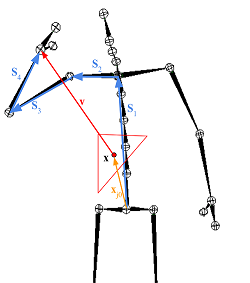
\includegraphics{../figures/SkeletonKinematicPath.png}
\caption{Kinematic Path}
\end{figure}

Molla computes the contribution of each bone segment \(\mathbf{s}_i\) in
the kinematic path to the position of the joint relative to the surface,
that is, the displacement vector \(\mathbf{v}\), based on the projection
of each bone vector onto the displacement vector by

\begin{equation}
\label{eq:contribution}
cos(\alpha_{i}) = \frac{\mathbf{v}}{||\mathbf{v}||}\cdot\frac{\mathbf{s}_{i}}{||\mathbf{s}_{i}||}
\end{equation}

The cosines of every bone in the kinematic path are kept as
\(C_{i} = \{|cos(\alpha_{1})|, |cos(\alpha_{2})|,..., |cos(\alpha_{n})|\}\)
for a kinematic path with \(n\) bone segments. To adapt the joint
position in the target skeleton, the displacement vector is normalized
as

\begin{equation}
\label{eq:tau}
\mathbf{\hat{v}} = \frac{\mathbf{v}}{\tau},\ where\ \tau = \sum_{i=0}^{n}||\mathbf{s}_{i}||\ |cos(\alpha_{i})|
\end{equation}

\emph{Summary}. Given a joint \(j\) and a surface component \(i\), we
store the set of parametes: \(\mathbf{e}_{j,i} = (\hat{\lambda}_{i}\),
\(\mathbf{\hat{v}}\), \(C_{i})\). The egocentric coordinates of a joint
\(E_{j}\) for a given frame considering all \(m\) surface components is
given by

\begin{equation}
\label{eq:egocoordsall}
E_{j} = \{e_{j,1}, e_{j,2},...,e_{j,m}\}
\end{equation}


    \subsection{Pose Adaptation}\label{pose-adaptation}

To adapt the pose of the target skeleton enforcing the same surface
spatial relationship as the souce motion, we denormalize the egocentric
coordinates with the parameters regarding the body proportions and bone
length of the target skeleton and surface. We compute the correct joint
position in the target skeleton of a extremity joint, then we use
Inverse Kinematics so that the skeleton reaches the new position.

First, we compute the reference point of each mesh component of the
target character using the surface estimation from Section Surface
Estimation. Then, we use the length of the bone segments to calculate
the importance factor \(\tau\) for the target skeleton and multiply it
by each normalized displacement vector \(\mathbf{\hat{v}}_{i}\).
Finally, the new position of the joint is given by Equation
\ref{eq:egocoord_jointpos2}.

\subsubsection{Inverse Kinematics}\label{inverse-kinematics}

We use the Jacobian Transpose method for the Inverse Kinematics (IK) to
compute the new pose of the avatar\cite{buss}. The kinematic paths fed
to the IK algorithm are composed of all joints from the beginning of the
limb to the limb extremity: the shoulder to the hand and the upper leg
to the foot. This allows a separete IK computing for each limb and
avoids dragging the spine and the hips in order to reach the target
position.

\subsection{Reproducible Research}\label{reproducible-research}

The algorithm developed during this work is available at
\href{https://github.com/rltonoli/MotionRetargeting/}{github}.

    \section{Results}\label{results}

Figure \ref{fig:result1} shows the pose of the source and target
skeletons of a motion capture take in which the actor is touching its
right eyebrow with his fingers. In the middle, the target animation is
the result of the bones alignment, where the red \(X\) indicates the
correct position of the right hand joint computed through the egocentric
coordinates. The Inverse Kinematis receives the pose and the correct
position and computes the new pose of the target skeleton, on the right.

Darker colors of blue represent a greater importance of the displacement
vectors. As expected from a movement close to the head, mesh componets
of the head are contributing more than those of the body. Furthermore,
the triangles with normal vectors pointing in the same direction as the
displacement vectors are also receiving greater weights, which indicates
that the orthogonality factor exposes possible interaction of the joints
with the surface.


    \captionsetup{labelformat=default}
    \begin{figure}
        \begin{center}\adjustimage{max size={1\linewidth}{0.4\paperheight}}{MotionRetargetingPaper-3_files/MotionRetargetingPaper-3_12_0.png}\end{center}
        \caption{Results.}
        \label{fig:result1}
    \end{figure}
    
    \section{Conclusion}\label{conclusion}

We applied the method described by Eray Molla to ensure the interaction
of the extremity joints with the body surface when retargeting motion
from Motion Capture data. With the body surfaces calibrated, the
algorithm computes a new pose for the target skeleton and uses Inverse
Kinematics to adapt the skeleton into the desired pose. We found that
the method is able to improve the target animation when the hands are
interacting with the body surface.

In future works, we wish to conduct a perpectual evaluation to assess
the resemblance between the target animations, adpated and non-adapted,
and the video of the Motion Capture actor performing the same movement.
Furthermore, towards sign language avatars, the work could be extended
to the fingers adaptation, since hand configuration is a key aspect on
sign characterization.


    % Add a bibliography block to the postdoc
    
    
\bibliographystyle{abbrv-doi}
\bibliography{reference}

    
    \end{document}
